%%%%%%%%%%%%%%%%%%%%%%%%%%%%%%%%%%%%%%%%%
% Short Sectioned Assignment
% LaTeX Template
% Version 1.0 (5/5/12)
%
% This template has been downloaded from:
% http://www.LaTeXTemplates.com
%
% Original author:
% Frits Wenneker (http://www.howtotex.com)
%
% License:
% CC BY-NC-SA 3.0 (http://creativecommons.org/licenses/by-nc-sa/3.0/)
%
%%%%%%%%%%%%%%%%%%%%%%%%%%%%%%%%%%%%%%%%%

%----------------------------------------------------------------------------------------
%	PACKAGES AND OTHER DOCUMENT CONFIGURATIONS
%----------------------------------------------------------------------------------------

\documentclass[paper=a4, fontsize=11pt]{scrartcl} % A4 paper and 11pt font size

\usepackage[T1]{fontenc} % Use 8-bit encoding that has 256 glyphs
\usepackage{fourier} % Use the Adobe Utopia font for the document - comment this line to return to the LaTeX default
\usepackage[english]{babel} % English language/hyphenation
\usepackage{amsmath,amsfonts,amsthm} % Math packages

\usepackage{lipsum} % Used for inserting dummy 'Lorem ipsum' text into the template

\usepackage{sectsty} % Allows customizing section commands
\allsectionsfont{\normalfont\scshape} % Make all sections centered, the default font and small caps
% \allsectionsfont{\centering \normalfont\scshape} % Make all sections centered, the default font and small caps

\usepackage{fancyhdr} % Custom headers and footers
\usepackage{graphicx}
\pagestyle{fancyplain} % Makes all pages in the document conform to the custom headers and footers
\fancyhead{} % No page header - if you want one, create it in the same way as the footers below
\fancyfoot[L]{} % Empty left footer
\fancyfoot[C]{} % Empty center footer
\fancyfoot[R]{\thepage} % Page numbering for right footer
\renewcommand{\headrulewidth}{0pt} % Remove header underlines
\renewcommand{\footrulewidth}{0pt} % Remove footer underlines
\setlength{\headheight}{13.6pt} % Customize the height of the header

\numberwithin{equation}{section} % Number equations within sections (i.e. 1.1, 1.2, 2.1, 2.2 instead of 1, 2, 3, 4)
\numberwithin{figure}{section} % Number figures within sections (i.e. 1.1, 1.2, 2.1, 2.2 instead of 1, 2, 3, 4)
\numberwithin{table}{section} % Number tables within sections (i.e. 1.1, 1.2, 2.1, 2.2 instead of 1, 2, 3, 4)

\setlength\parindent{0pt} % Removes all indentation from paragraphs - comment this line for an assignment with lots of text

%----------------------------------------------------------------------------------------
%	TITLE SECTION
%----------------------------------------------------------------------------------------

\newcommand{\horrule}[1]{\rule{\linewidth}{#1}} % Create horizontal rule command with 1 argument of height

\title{	
\normalfont \normalsize 
\textsc{CSIT 6000F} \\ [25pt] % Your university, school and/or department name(s)
\horrule{0.5pt} \\[0.4cm] % Thin top horizontal rule
\huge Assignment 1 \\ % The assignment title
\horrule{2pt} \\[0.5cm] % Thick bottom horizontal rule
}

\author{Yuchen, GUO   No.20477118} % Your name

\date{\normalsize September 20, 2017} % Today's date or a custom date

\begin{document}

\maketitle % Print the title

%----------------------------------------------------------------------------------------
%	PROBLEM 1
%----------------------------------------------------------------------------------------

\section{Problem 1}

In this problems, we can describe the input of the sensors using a matrix:

\begin{align*}
S = 
\begin{bmatrix}
    s_1 & s_2 & s_3\\
    s_8 & - & s_4\\
    s_7 & s_6 & s_5
\end{bmatrix}
\end{align*}

So the robot has only 9 exclusive states as following:

\begin{align*}
S_1 = 
\begin{bmatrix}
    1 & 1 & 1\\
    1 & - & 0\\
    1 & 0 & 0
\end{bmatrix},
S_2 = 
\begin{bmatrix}
    1 & 1 & 1\\
    0 & - & 0\\
    0 & 0 & 0
\end{bmatrix},
S_3 = 
\begin{bmatrix}
    1 & 1 & 1\\
    0 & - & 1\\
    0 & 0 & 1
\end{bmatrix},\\
S_4 = 
\begin{bmatrix}
    1 & 0 & 0\\
    1 & - & 0\\
    1 & 0 & 0
\end{bmatrix},
S_5 = 
\begin{bmatrix}
    0 & 0 & 0\\
    0 & - & 0\\
    0 & 0 & 0
\end{bmatrix},
S_6 = 
\begin{bmatrix}
    0 & 0 & 1\\
    0 & - & 1\\
    0 & 0 & 1
\end{bmatrix},\\
S_7 = 
\begin{bmatrix}
    1 & 0 & 0\\
    1 & - & 0\\
    1 & 1 & 1
\end{bmatrix},
S_8 = 
\begin{bmatrix}
    0 & 0 & 0\\
    0 & - & 0\\
    1 & 1 & 1
\end{bmatrix},
S_9 = 
\begin{bmatrix}
    0 & 0 & 1\\
    0 & - & 1\\
    1 & 1 & 1
\end{bmatrix},
\end{align*}

The state of every cell is shown in Figure ~\ref{fig:Problem1.1.1}.\\
\\
\begin{figure}[h]
    \centering
    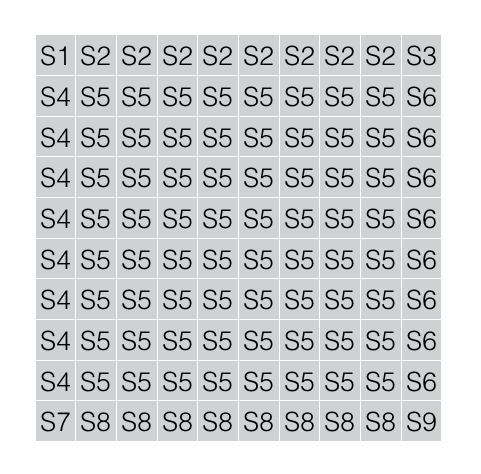
\includegraphics[scale=0.5]{image7.png}
    \caption{State of every cell in the grid.}
    \label{fig:Problem1.1.1}
\end{figure}\\

Below are the boolean forms of $S_1$ to $S_9$:

\begin{align*}
S_1 = s_1 \cdot s_2 \cdot s_3 \cdot \overline{s_4} \cdot \overline{s_5} \cdot \overline{s_6} \cdot s_7 \cdot s_8\\
S_2 = s_1 \cdot s_2 \cdot s_3 \cdot \overline{s_4} \cdot \overline{s_5} \cdot \overline{s_6} \cdot \overline{s_7} \cdot \overline{s_8}\\
S_3 = s_1 \cdot s_2 \cdot s_3 \cdot s_4 \cdot s_5 \cdot \overline{s_6} \cdot \overline{s_7} \cdot \overline{s_8}\\
S_4 = s_1 \cdot \overline{s_2} \cdot \overline{s_3} \cdot \overline{s_4} \cdot \overline{s_5} \cdot \overline{s_6} \cdot s_7 \cdot s_8\\
S_5 = \overline{s_1} \cdot \overline{s_2} \cdot \overline{s_3} \cdot \overline{s_4} \cdot \overline{s_5} \cdot \overline{s_6} \cdot \overline{s_7} \cdot \overline{s_8}\\
S_6 = \overline{s_1} \cdot \overline{s_2} \cdot s_3 \cdot s_4 \cdot s_5 \cdot \overline{s_6} \cdot \overline{s_7} \cdot \overline{s_8}\\
S_7 = s_1 \cdot \overline{s_2} \cdot \overline{s_3} \cdot \overline{s_4} \cdot s_5 \cdot s_6 \cdot s_7 \cdot s_8\\
S_8 = \overline{s_1} \cdot \overline{s_2} \cdot \overline{s_3} \cdot \overline{s_4} \cdot s_5 \cdot s_6 \cdot s_7 \cdot \overline{s_8}\\
S_9 = \overline{s_1} \cdot \overline{s_2} \cdot s_3 \cdot s_4 \cdot s_5 \cdot s_6 \cdot s_7 \cdot \overline{s_8}\\
\end{align*}

%------------------------------------------------

\subsection{}

Let's take the northwest corner for example.\\

When the robot is not next to the north border, move it to north, otherwise move it to west\\

Here is the production system:\\

\boldmath \begin{align*}
&\overline{s_2} \longrightarrow north\\
&\overline{s_8} \longrightarrow west
\end{align*}
or
\boldmath \begin{align*}
&S_2+S_3 \longrightarrow west\\
&S_4+S_5+S_6+S_7+S_8+S_9 \longrightarrow north
\end{align*}

%------------------------------------------------

\subsection{}

We can prove it by putting the robot in the center of the grid, 
and then prove it can't visit every cell. Here are my two methods:\\

\subsubsection{Method One}

With $S_5$, it can move in any direction in ${north, west, east, south}$, 
in Figure ~\ref{fig:Problem1.2.1}, 
we assume it be west, and it can be any direction by rotating the image, 
the situations are equivalent.

The robot will move in the same direction until it reaches a border.
To visit all cells in the grid, it must visit other cells with $S_5=1$.
So let's see how can its state transfer to $S_5$ again,
all possible ways are marked with pointers in the left part of Figure ~\ref{fig:Problem1.2.1}.
So in every path it enters a $S_5$ cell, it will go straight to the west border and 
can't visit other $S_5$ cells, so it's proved that no production system 
can make the robot visit all cells in the grid.
The right part shows possible circles that the robot can move in(equivalent paths are ignored).\\
    
\begin{figure}[p]
    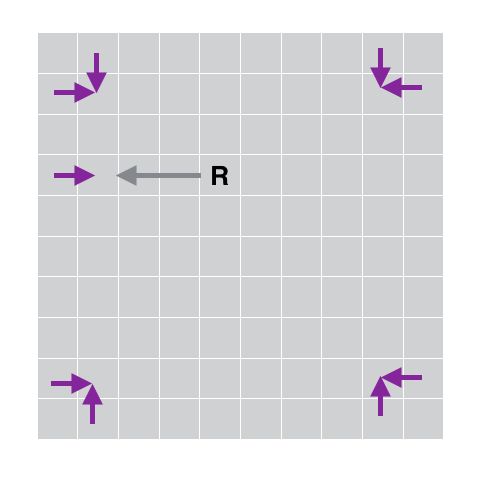
\includegraphics[scale=0.5]{image1.png}
    \hspace{\fill}
    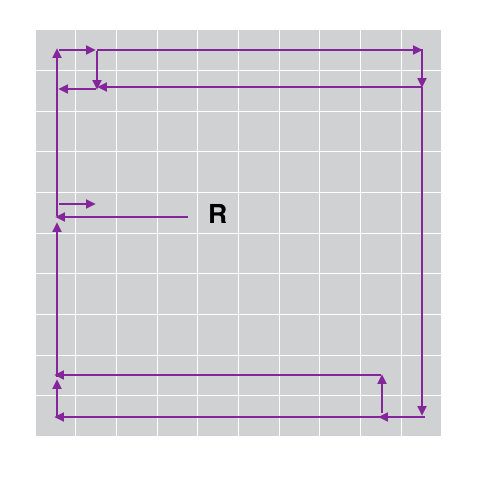
\includegraphics[scale=0.5]{image2.png}
    \caption{Ways to enter $S_5$ again and possible circles}
    \label{fig:Problem1.2.1}
    \vspace{\fill}
    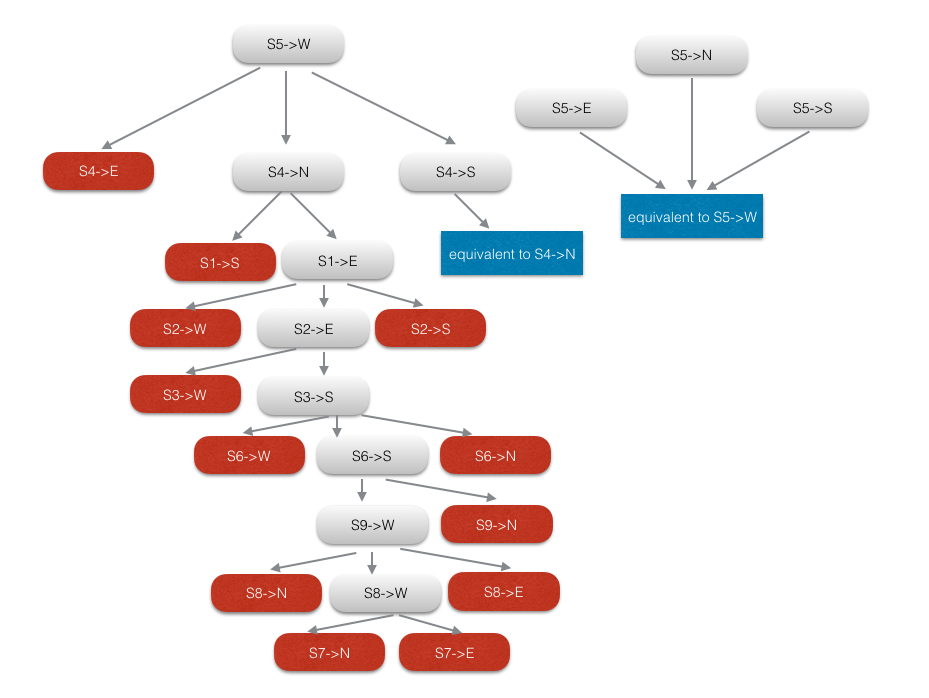
\includegraphics[scale=0.5]{image6.png}
    \caption{Search tree to find production system that can visit all cells, 
        red nodes means the robot is going to move in a circle of several nodes,
        blue nodes means the situation is equivalent to another one, as we can see,
        all paths ends with a red node.}
    \label{fig:Problem1.2.2}
\end{figure}

\subsubsection{Method Two}

Figure ~\ref{fig:Problem1.2.2} shows all production systems makes the robot move between 
some cells(Not all cells in the grid).\\

The search tree expands in the following process:\\

We start with a $S_5$ cell, four actions are in fact equivalent as we rotate the grid, 
assume the production system gives $S_5 \rightarrow W$, it reaches the west border,
the next decision is $S_4 \rightarrow ?$. \\

If $S_4 \rightarrow E$, the robot will move between two nodes. \\
So we just need to expand $S_4 \rightarrow N$ and $S_4 \rightarrow S$,
and the two branches are equivalent too. Let's assume $S_4 \rightarrow N$.\\

Then the robot reaches the northwest corner: $S_1$, \\
If $S_1 \rightarrow S$, the robot will move between two nodes. \\
So $S_1 \rightarrow E$.\\

Then the state of the robot becomes $S_2$, \\
If $S_2 \rightarrow W$, the robot will move between two nodes. \\
If $S_2 \rightarrow S$, the robot will move in a circle of four nodes. \\
So $S_2 \rightarrow E$.\\

Then the state of the robot becomes $S_3$, \\
If $S_3 \rightarrow W$, the robot will move between two nodes. \\
So $S_3 \rightarrow S$.\\

Then the state of the robot becomes $S_6$, \\
If $S_6 \rightarrow N$, the robot will move between two nodes. \\
So $S_6 \rightarrow W$, the robot will move in a circle of twenty nodes. \\
So $S_6 \rightarrow S$.\\

Then the state of the robot becomes $S_9$, \\
If $S_9 \rightarrow N$, the robot will move between two nodes. \\
So $S_9 \rightarrow W$.\\

Then the state of the robot becomes $S_8$, \\
If $S_8 \rightarrow E$, the robot will move between two nodes. \\
So $S_8 \rightarrow N$, the robot will move in a circle of thirty-six nodes. \\
So $S_8 \rightarrow W$.\\

Then the state of the robot becomes $S_7$, \\
If $S_7 \rightarrow E$, the robot will move between two nodes. \\
So $S_7 \rightarrow N$.\\

So, the state of the robot becomes $S_4$ again, it will move clockwise next to the border, 
move in a circle of thirty-six nodes.\\

Thus it's proved that no production system can make the robot visit all cells in the grid. \\

%------------------------------------------------
\subsection{Part 3 of Problem 1}

Let $W_{ij}$ be the features defined as:\\
$W_{ij}$ = 1 iff at the previous time step, $S_i$ = 1, and the robot moved $j$($j \in \{N, W, E, S\}$).
For example:
$W_{1E}$ = 1 iff at the previous time step, $S_1$ = 1, and the robot moved $East$.\\

\begin{figure}[h]
    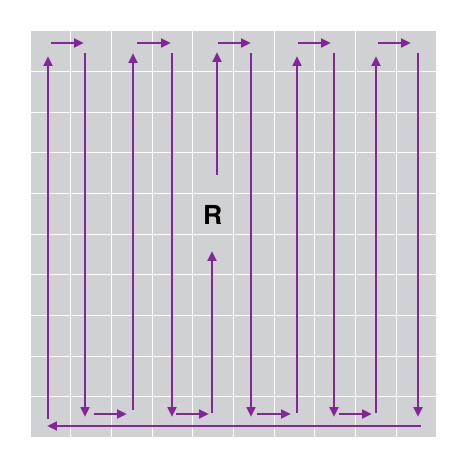
\includegraphics[scale=0.5]{image3.png}
    \hspace{\fill}
    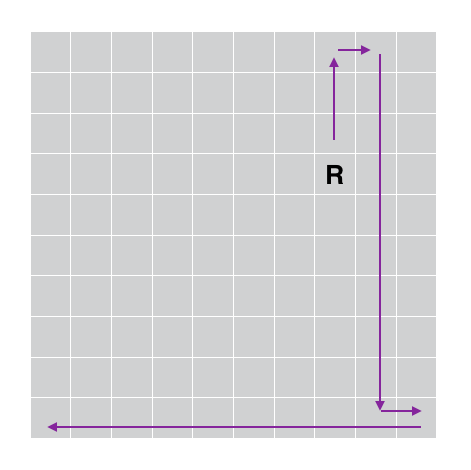
\includegraphics[scale=0.5]{image4.png}
    \caption{Two situations to visit all cells}
    \label{fig:Problem1.3}
\end{figure}

As Figure ~\ref{fig:Problem1.3} shows, we want the robot to visit every cell 
in the route in the left picutre.

Here is the production system:
\boldmath \begin{align*}
&S_2 \cdot W_{5N} \longrightarrow east\\
&S_2 \cdot (W_{2E} + W_{1E}) \longrightarrow south\\
&S_5 \cdot (W_{2S}+W_{5S}) \longrightarrow south\\
&S_5 \cdot (W_{8N}+W_{5N}) \longrightarrow north\\
&S_8 \cdot W_{5S} \longrightarrow east\\
&S_8 \cdot W_{8E} \longrightarrow north\\
&S_8 \cdot (W_{8W}+W_{9W}) \longrightarrow west\\
&S_1 \longrightarrow east\\
&S_3+S_6 \longrightarrow south\\
&S_4+S_5+S_7 \longrightarrow north\\
&S_9 \longrightarrow west\\
&1 \longrightarrow north
\end{align*}

%----------------------------------------------------------------------------------------
%	PROBLEM 2
%----------------------------------------------------------------------------------------

\section{Problem 2}

Let the input be $A, B, C, D, E$. Then:

\begin{align*}
Result=(1.1*A+3.1*B-C-2*D+0.5*E>1)\\
\end{align*}

Accoding to the inequation above:\\
If $C \cdot D$, $Result=1$ iff $1.1*A+3.1*B+0.5*E>4$ iff $A \cdot B$\\
If $C \cdot \overline{D}$, $Result=1$ iff $1.1*A+3.1*B+0.5*E>2$ iff $B$\\
If $\overline{C} \cdot D$, $Result=1$ iff $1.1*A+3.1*B+0.5*E>3$  iff $B$\\
If $\overline{C} \cdot \overline{D}$, $Result=1$ iff $1.1*A+3.1*B+0.5*E>1$ iff $A + B$\\

So:

\begin{align*}
Result&= C \cdot D \cdot A \cdot B + 
         C \cdot \overline{D} \cdot B +
         \overline{C} \cdot D \cdot B +
         \overline{C} \cdot \overline{D} \cdot (A + B)\\
      &= A \cdot B \cdot C \cdot D + 
         A \cdot \overline{C} \cdot \overline{D} +
         B \cdot (\overline{C} \cdot \overline{D} + C \cdot \overline{D} + \overline{C} \cdot D)\\
      &= A \cdot B \cdot C \cdot D + 
         (A + 1) \cdot B \cdot (\overline{C} \cdot \overline{D} + C \cdot \overline{D} + \overline{C} \cdot D) +
         A \cdot \overline{C} \cdot \overline{D}\\
      &= A \cdot B \cdot C \cdot D + 
         A \cdot B \cdot (\overline{C} \cdot \overline{D} + C \cdot \overline{D} + \overline{C} \cdot D) +
         B \cdot (\overline{C} \cdot \overline{D} + C \cdot \overline{D} + \overline{C} \cdot D) +
        %  B \cdot (\overline{C} + \overline{D}) +
         A \cdot \overline{C} \cdot \overline{D} \\
      &= A \cdot B \cdot (C \cdot D + \overline{C} \cdot \overline{D} + C \cdot \overline{D} + \overline{C} \cdot D) +
         A \cdot \overline{C} \cdot \overline{D} +
         B \cdot (\overline{C} + \overline{D})\\
      &= A \cdot B +
         A \cdot \overline{C} \cdot \overline{D} +
         B \cdot (\overline{C} + \overline{D}) 
\end{align*}

%----------------------------------------------------------------------------------------

%----------------------------------------------------------------------------------------
%	PROBLEM 3
%----------------------------------------------------------------------------------------

\section{Problem 3}

As Figure ~\ref{fig:Problem3.1} shows, we can use Breadth First Search to find the minimal set of training instances. 
The depth of the search tree is the size of the training set, so we can always get the minimal set.

\begin{figure}[h]
    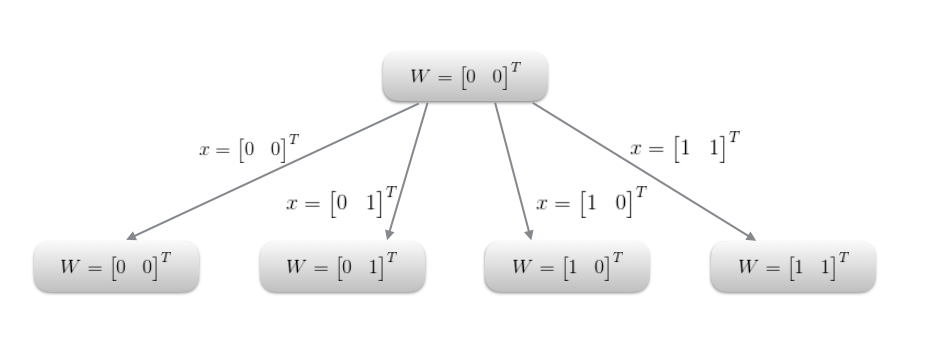
\includegraphics[scale=0.5]{image5.png}
    \caption{Breadth-first search to do error-correction}
    \label{fig:Problem3.1}
\end{figure}

\begin{figure}[t]
    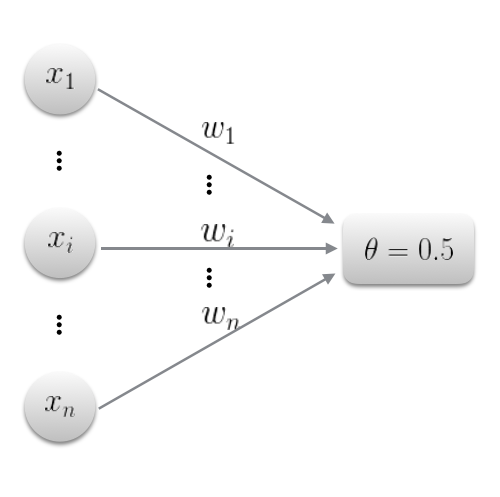
\includegraphics[scale=0.4]{image8.png}
    \hspace{\fill}
    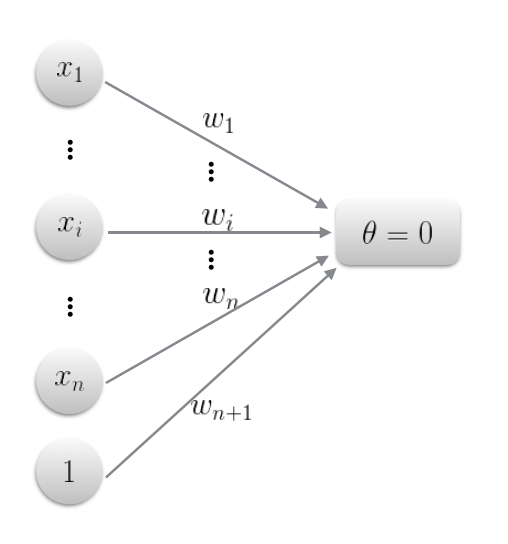
\includegraphics[scale=0.4]{image9.png}
    \caption{TLU without augmented vectors and TLU with augmented vectors}
    \label{fig:Problem3.2}
\end{figure}

\subsection{Without augmented vectors}

As the left part of Figure ~\ref{fig:Problem3.2} show, we have a preassigned $\theta=0.5$.\\

We have learning rate $c=1$, 
and $w$ is inited as $w_0=\begin{bmatrix}0 & 0 & ... & 0 & 0\end{bmatrix}$.\\

% so for whatever train data $x_1$ in the first iteration, 
% we have $f=w_0x_1=0$
If $x_1=\begin{bmatrix}0 & 0 & \cdots & 0 & 0\end{bmatrix}$, then $d_1=0$,
$f_1=w_0x_1^T=0 \leqslant 0.5$,
$w_1=w_0+1*(0-0)*x_1 = w_0$, $w$ didn't change, the model is not improved.\\

If $x_1=\begin{bmatrix}x_{1, 1} & x_{1, 2} & \cdots & x_{1, n-1} & x_{1, n}\end{bmatrix}$ 
    ($\exists i \in [1, n], x_{1, i} \neq 0$), then $d_1=1$, 
$f_1=w_0x_1^T=0 \leqslant 0.5$, $w_1=w_0+1*(1-0)*x_1 = x_1$.\\

We can find that, if $x_1=\begin{bmatrix}1 & 1 & \cdots & 1 & 1\end{bmatrix}=w_1$, 
all inputs can get the correct result.\\

So the minimal set of training instances is $\{\begin{bmatrix}1 & 1 & \cdots & 1 & 1\end{bmatrix}\}$

\subsection{With augmented vectors}

As the right part of Figure ~\ref{fig:Problem3.2} show, we have a constant input $\forall i, x_{i,n+1}=1$.\\

We have learning rate $c=1$, and a default threshold $\theta=0$, 
and $w \in R^{n+1}$ is inited as $w_0=\begin{bmatrix}0 & 0 & ... & 0 & 0\end{bmatrix}$.\\

% so for whatever train data $x_1$ in the first iteration, 
% we have $f=w_0x_1=0$
If $x_1=\begin{bmatrix}0 & 0 & \cdots & 0 & 1\end{bmatrix}$, then $d_1=0$,
$f_1=w_0x_1^T=0 \leqslant 0$,
$w_1=w_0+1*(0-0)*x_1 = w_0$, $w$ didn't change, the model is not improved.\\

If $x_1=\begin{bmatrix}x_{1, 1} & x_{1, 2} & \cdots & x_{1, n} & x_{1, n+1}\end{bmatrix}$ 
    ($\exists i \in [1, n], x_{1, i} \neq 0$), then $d_1=1$, 
$f_1=w_0x_1^T=0 \leqslant 0$, $w_1=w_0+1*(1-0)*x_1 = x_1$.\\

We can find that, if $x_1=\begin{bmatrix}1 & 1 & \cdots & 1 & 1\end{bmatrix}=w_1$, 
all inputs except $\begin{bmatrix}0 & 0 & \cdots & 0 & 0 & 1\end{bmatrix}$ can get the correct result.\\

So let $x_2=\begin{bmatrix}0 & 0 & \cdots & 0 & 0 & 1\end{bmatrix}$, then $d_2=0$,
$f_2=w_1x_2^T=1>0$,
$w_2=w_1+1*(0-1)*x_1=\begin{bmatrix}1 & 1 & \cdots & 1 & 1 & 0\end{bmatrix}$.\\

Here $w_2$ perfectly output the "or" result for any input.\\

So the minimal set of training instances is $\{\begin{bmatrix}1 & 1 & \cdots & 1 & 1\end{bmatrix},
\begin{bmatrix}0 & 0 & \cdots & 0 & 0\end{bmatrix}\}$

%----------------------------------------------------------------------------------------

%----------------------------------------------------------------------------------------
%	PROBLEM 4
%----------------------------------------------------------------------------------------

\section{Problem 4}

\subsection{}

The input of the fitness function is an algorithm that moves the elevator to take people to the correct floor.

The output of the fitness function is total floors the elevator moved in the process of moving everyone to their target floor.

Algorithms with less total floor should be selected as the next generation.

\subsection{}

The input of the fitness function is the algorithm that changes the traffic lights at the intersection.

The output of the fitness function is total time all vehicles and passerbys waited at the crossroad.

Algorithms with less total time should be selected as the next generation.

%----------------------------------------------------------------------------------------

%----------------------------------------------------------------------------------------
%	PROBLEM 5
%----------------------------------------------------------------------------------------

\section{Problem 5}

Feature:\\
$F_1$: cricket is on the threshold, $\overline{F_1}$ means the cricket is away from the threshold\\
$OK$: ok bit used to remember whether it's ok inside

Action:\\
$A_1$: go to the cricket and move it to the threshold\\
$A_2$: go inside and check, then return to the threshold\\
$A_3$: drag the cricket inside\\

Production System:\\
\begin{align*}
\overline{F_1} &\longrightarrow A_1, OK=0\\
F_1 \cdot \overline{OK} &\longrightarrow A_2, OK=1\\
F_1 \cdot OK &\longrightarrow A_3\\
\end{align*}



%----------------------------------------------------------------------------------------
\end{document}